\titre{Arbre ordonné} \\
$\left\{ \begin{array}{l}
	\vide \in V \\
	\forall (x_1,\ldots , x_n)  \in X \; \mathrm{liste}\;\mathrm{ordonnee}, \forall v \in V, (v,x_1,\ldots,x_n) \in X
\end{array} \right.$  \\

\par

\titre{Arbre binaire} \\
$\left\{ \begin{array}{l}
	\vide \in A \\
	\forall A_g,A_d \in A, r\in X, (A_g,r,A_d)\in A
\end{array} \right.$ \\

\par

\titre{Arbre binaire étiqueté par un ensemble $A$} \\
$\left\{ \begin{array}{l}
	\vide \in AB \\
	\forall g,d \in AB, \forall a \in A, (g,a,d)\in AB 
\end{array}
\right.$\\

\par

\titre{ATTENTION} Les deux arbres ci-dessous sont les mêmes arbres ordonnés, mais pas les mêmes arbres binaires : \\
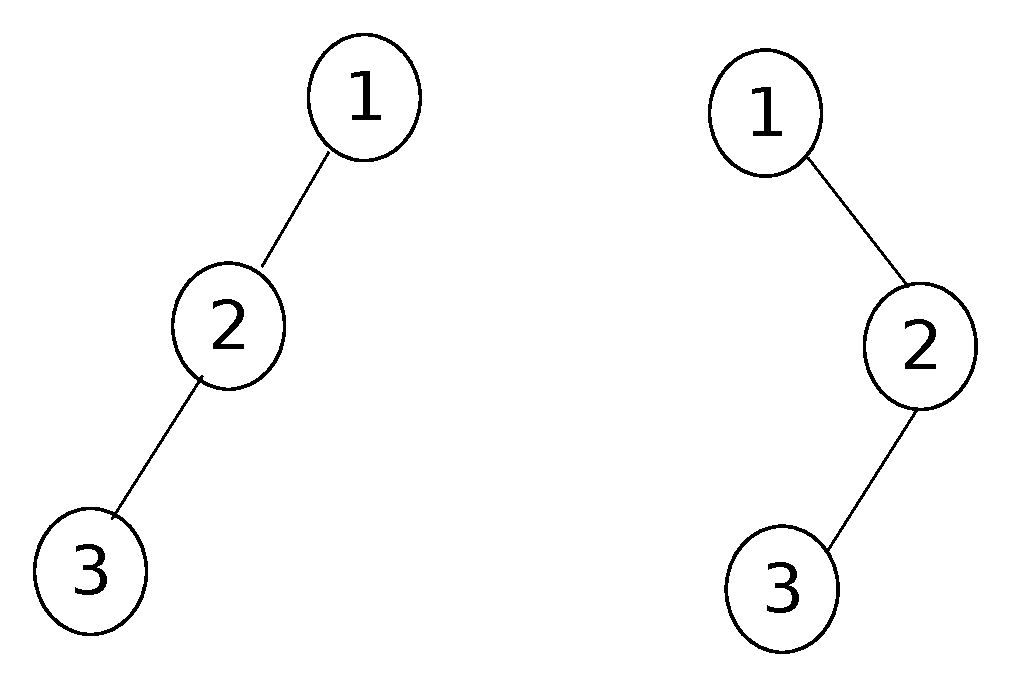
\includegraphics[width=5cm]{D4_1.pdf} \\
Arbre de gauche : $(((\vide,3,\vide),2,\vide),1,\vide)$ \\
Arbre de droite : $(\vide,1,((\vide,3,\vide),2,\vide)$
